\chapter{クラスの例}
\section{例の概要}
図\ref{color}はここで示す例の表示画面である。
\begin{figure}[ht]
 \begin{center}
  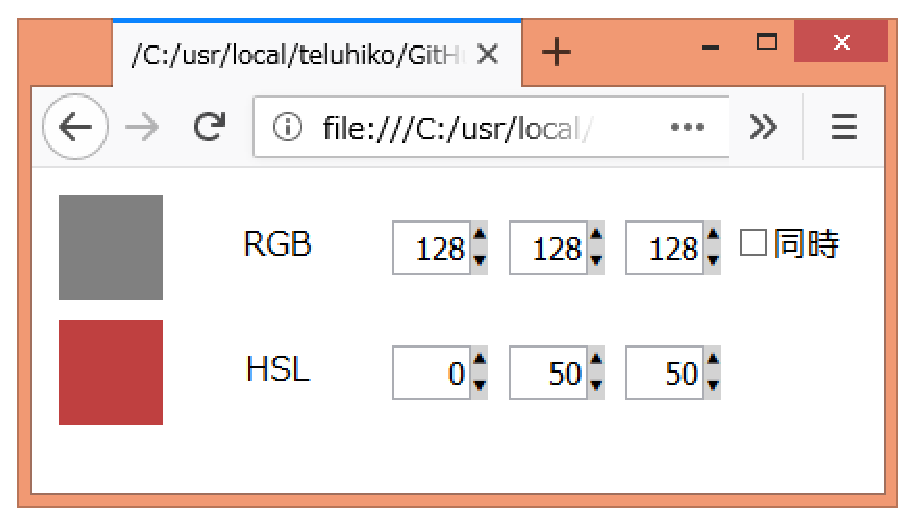
\includegraphics[width=0.5\textwidth]{13Ex.eps}
 \end{center}
 \caption{色の指定を見る}\label{color}
\end{figure}

この例では上下2行のテキストボックスで指定された色を左側の正方形の部分で
示す。上はRGB形式で、下はHSL\footnote{W3CのCSS Color Module Level
3\texttt{https://www.w3.org/TR/2011/REC-css3-color-20110607/}を参照のこ
と}形式で色を指定することができる。色を変える操作は次のとおりである。
\begin{itemize}
 \item それぞれのテキストボックスの値は▲をクリックすると増加し、▼をクリッ
       クすると1ずつ減少する。シフトキーを押しながらクリックすると5ずつ
       変化する。
 \item RGB形式の値は$0\sim255$の間で変化する。上限または下限の範囲を超え
       る場合は上限または下限の値にとどまる。一番右のチェックボックスに
       チェックがあると3つの値が同時に増減する。
 \item HSL形式の値は一番左(H--色相)が$0\sim359$の間で循環して変化し、残
       りの2つは$0\sim100$の間で変化する。
\end{itemize}
\section{ソースコードの解説}
\subsection{HTMLファイル}
次のリストはHTMLファイルのものである。
\LISTN{13Ex.html}{1}{last}{\normalsize}
\begin{itemize}
 \item 5行目ではこのページに関する処理を定義する\JS ファイル
       (\texttt{13Ex.js})を、
 % \item
			 6行目ではユーザーインターフェイスを定義している\JS ファイル
       (\texttt{13UI.js})を読み込む。
 \item 7行目から15行目は色を表示する部分のCSSを定義している。
       \begin{itemize}
        \item 9行目と10行目では表示部分の大きさ
        \item 11行目では配置方法(横に並べる)
        \item 12行目では上下の位置(ここでは中央に指定)
        \item 13行目では色の表示域の周りの空白
       \end{itemize}
 \item 18行目と19行目では色の表示位置と値を設定するための\texttt{<div>}
       要素を定義している。
\end{itemize}
 \subsection{ユーザーインターフェイス}
 次のリストはユーザーインターフェイスのクラスを定義するものである。

次のリストの部分は指定されたオブジェクトに指定できるオプションの値を変更するた
 めの関数を定義している。
 \LISTN{13UI.js}{1}{5}{\normalsize}
\begin{itemize}
 \item 2番目の引数(\texttt{Opt})は変更する値が入っているオブジェクトであ
       る。
 \item 1番目の引数はキーがオブジェクト内の指定できるオプション(デフォル
       ト値が設定されている)からなるオブジェクトである。
 \item 3行目で指定できるキーであれば値を設定している。
\end{itemize}
次のリストの部分はHTML要素に対する\texttt{style}を設定するための関数である。
\LISTN{13UI.js}{6}{9}{\normalsize}
\begin{itemize}
 \item 7行目で、指定されたオプションを設定している。
 \item 8行目でオプションのオブジェクトを\texttt{style}属性の形式になるよ
       うに、オブジェクトを\texttt{JSON}形式の文字列に変換した後、
 キーなどを囲む\texttt{\{}と\texttt{"}を取り除き、%"
 \texttt{,}と\texttt{\}}を\texttt{;}に変換している。
\end{itemize}
10行目から35行目のリストの部分は基本となるオブジェクト\texttt{DOMObject}を定義
している。
\LISTN{13UI.js}{10}{35}{\normalsize}
\begin{itemize}
 \item オブジェクト内で有効な定数を定義するためにクラス式を返す関数を定
       義しその場で実行している(35行目の\texttt{()})。
 \item 11行目から14行目で作成する要素の名前空間のリストをオブジェクトリ
       テラルの形で定義している。ここではHTML要素とSVG要素の名前空間があ
       る。
 \item 16行目から18行目で\texttt{document.getElementById()}の相当する
       このオブジェクト用の関数を定義している。
 \item 19行目から23行目で\texttt{document.getElementsByTagName()}の相当する
       このオブジェクト用の関数を定義している。
       \begin{itemize}
        \item 20行目で指定された要素のリストを得ている。
        \item 21行目から22行目でそのリストを\texttt{DOMObject}のリストに
              変更している。
        \item \ElmJ{map}は配列オブジェクト\ElmJ{Array}のメソッドで、各要
              素に対して引数で与えられた関数を実行し、その結果からなる配
              列を返す。
        \item 20行目で得られたリストは配列ではないのでこのメソッドを使用
              できない。
        \item \ElmJ{call}は指定した関数が参照する\ElmJ{this}をその1番目
              の引数にする。
        \item 22行目の\texttt{(E)}以降の書き方は新しい無名関数の
              記述方法である。\Verb+function(E){...}+
              と書くのと同じである。
        \item 新しい書き方と従来の書き方の一番の違いは関数内での
              \ElmJ{this}の取り扱いである。\ElmJ{class}内のコードは
              \texttt{strict}モードで実行される。このとき、
              \ElmJ{function}で定義された関数内では\ElmJ{this}は
              \ElmJ{undefined}になる。一方、簡略化された記述では
              \ElmJ{this}の値がオブジェクト自身を指す。この違いが問題と
              なる例はこのリストの141行目などにある。
       \end{itemize}
 \item 24行目から31行目はこのオブジェクトの\ElmJ{constructor}を定義して
       いる。
       \begin{itemize}
        \item 引数は順に作成する要素名、その属性のリスト、親要素、イベン
              ト処理のリスト、名前空間(デフォルトはHTML)である。
        \item 26行目で名前空間を指定して要素を作成している。
        \item 27行目は作成した要素に、与えられた属性を設定する関数を呼び
              出している。
        \item 28行目では親要素がある場合にはその子要素になるよ
              うに指定している。
        \item 29行目ではイベント処理を設定している。
        \item 32行目から34行目では与えられたリストの属性を設定する関数を
              定義している。
       \end{itemize}
\end{itemize}
次のリストの部分は与えられた文字列を表示するためのクラス\texttt{divWithText}を
定義している。
\LISTN{13UI.js}{36}{41}{\normalsize}
\begin{itemize}
 \item このクラスは\texttt{DOMObject}を継承している。
 \item コンストラクタの引数は順に、表示するテキスト、親要素、属性である。
 \item 39行目で\texttt{<div>}要素を作成し、その要素の\ElmJ{innerText}プロパティを
       設定することで表示を可能としている
\end{itemize}
\iffalse
class NamedTextBox extends divWithText{
  constructor(name, P, size="5", initValue=""){
    super(name, P, {style:"display:inline-block;margin:5px"});
    this.textBox = new DOMObject("input",
         {type:"text", style:"text-align:right",
          size:size, value:initValue},this);
  }
  get value(){return this.textBox.elm.value;}
}

次のリストの部分は与えられた文字列を表示し、そのあとにテキストボックスを
表示するためのクラス\texttt{NamedTextBox}を定義している。
\LISTN{13UI.js}{50}{58}{\normalsize}
\begin{itemize}
 \item このクラスは\texttt{divWithText}を継承している。
 \item コンストラクタの引数は順に、表示するテキスト、親要素、テキストボックス
       の大きさとその初期値である(51行目)。
 \item 作成した\texttt{<div>}要素の子要素にテキストボックスを作成してい
       る(53行目から55行目)。
 \item 57行目でテキストボックスの値を読み出すゲッター\texttt{value}を定
       義している。
\end{itemize}
\fi
\iffalse
class Button extends divWithText{
  constructor(name, P, E){
    super("", P);
    this.button = new DOMObject("input", {type:"button", value:name},this, E);
  }
  get value(){return this.button.elm.value;}
}

次のリストの部分はボタンクラスを作成するものである。
\LISTN{13UI.js}{50}{54}{\normalsize}
\begin{itemize}
 \item このクラスは\texttt{divWithText}を継承している。
 \item コンストラクタの引数は順に、ボタンに表示するテキスト、親要素、ボ
       タンのイベント処理関数のリストである(60行目)。
 \item 61行目で親要素の設定を行っている。
 \item 62行目でボタン要素を付け加えている。
\end{itemize}
\fi
42行目からのリストの部分はテキストボックスに付属した値を上下するボタンを持つ
\texttt{spinbox}のクラスを定義している。HTMLにも\texttt{spinbox}があるが
少し機能を変えている。

次のリストはこのクラスのコンストラクタの部分である。
\LISTN{13UI.js}{42}{73}{\normalsize}
\begin{itemize}
 \item コンストラクタの引数は順に、オプション、親要素、イベント処理関数
       群、値が変化したときの処理関数である。
 \item 44行目は値が変化したときに呼び出される関数をオブジェクトに登録し
       ている。
 \item 45行目から49行目ではこのオブジェクトのデフォルトのパラメータを定
       義している。
       \begin{itemize}
        \item \texttt{max}は設定できる値の最大値(デフォルト値は
              JavaScriptで扱うことができる最大値)
        \item \texttt{mix}は設定できる値の最小値(デフォルト値は
              JavaScriptで扱うことができる最小値)
        \item \texttt{skip}は値の変化量(デフォルト値は$1$)
        \item \texttt{bigSkip}はシフトキーを押しながらクリックしたときの
              値の変化量(デフォルト値は$5$)
        \item \texttt{value}は初期値(デフォルト値は$0$)
        \item \texttt{type}は両端の値から外れたときの処理方法(デフォルト
              は両端の値に固定--\texttt{"limited"}。値が循環的に変わる
              \texttt{"cyclic"}がある)
       \end{itemize}
 \item 50行目でオブジェクトの周りの余白の設定をしている。
 \item 51行目で入れ物の\texttt{<div>}要素を作成している。
 \item 52行目では45行目からのデフォルトのパラメータを与えられた値に変更
       している。
 \item 53行目から55行目では56行目から58行目で定義されるテキストボックス
       を入れるための\texttt{<div>}要素を作成している。
 \item 56行目から58行目で定義されるテキストボックスは\texttt{"readonly"}
       属性により値変更を直接できない。
 \item 59行目から60行目ではテキストボックスの隣に置く上下のボタンを入れ
       るための\texttt{<div>}要素を作成している。
 \item 61行目から64行目では値の上下させるボタンの表示形式を定義している。
 \item 65行目でさらにボタンのタイプ(値を増加)を設定し、66行目から67行目でボタンと
       して機能するようなオブジェクトを追加している。この上でクリックイ
       ベントが生じたときにイベント発生時ののシフトキーの状態を
       \texttt{sipnbox}の\texttt{up}プロパティの与えている(代入で行って
       いるが、\texttt{up}は76行目から85行目で定義されているセッターで
       ある)。
 \item 69行目から72行目は値を減少させるボタンを設定している。
\end{itemize}
残りの部分はこのクラスのセッターまたはゲッターを定義している部分である。
\LISTN{13UI.js}{74}{96}{\normalsize}
\begin{itemize}
 \item 74行目と75行目はそれぞれテキストボックスの値に関するゲッ
       ターとセッターである。
 \item 76行目から85行目は設定値を増大させるメソッドであり、86行目から
       95行目は設定値を減少させるメソッドである。
 \item 77行目ではシフトキーが押されているかを判定して、変化量を決めてい
       る。
 \item 78行目で仮の値を求め、それが上限値を超えている処理を79行目から
			 83行目で行っている。
 % \item
			 上限値で固定(\texttt{type}が\texttt{"limited"})のときは
       上限値と仮の値の小さい方を設定している(80行目)。
% \item
			値が循環する(\texttt{type}が\texttt{"cyclic"})ときは
       上限値が超えた場合、上限値の値を引いている(82行目)。
 \item 値の設定後の処理関数が定義されているときはその関数を呼び出す(84
       行目)。
 \item 値が減少する場合も同様である。
\end{itemize}
リストの最後の部分は色の3成分を設定するクラスの定義である。
\LISTN{13UI.js}{97}{last}{\normalsize}
\begin{itemize}
 \item コンストラクタに引数は順に、左端に示すテキスト、RGB形式かHSL形式
			 のタイプ、親要素、値が変化したときの処理関数、オブジェクトのオプ
			 ションである。
 \item 99行目のコメント行は、メソッド内で呼び出される無名関数内でオブ
			 ジェクト自身を示す\ElmJ{this}が参照できないときの対処法である。
			 \ElmJ{this}を変数(\texttt{that})に格納し、それを参照する。
 \item 101行目から104行目は左端にテキストが表示されるようにしている。
 \item 105行目から128行目ではタイプが\texttt{"rgb"}のときのオブジェク
			 トを作成している。
			 \begin{itemize}
				\item 106行目でタイプを\texttt{"rgb"}に設定している。
				\item 107行目から116行目でオブジェクト全体を囲む要素を作成して、
							そこに\texttt{click}イベントの処理関数を定義している。
				\item このオブジェクトの右端のチェックボックス(125行目から116行
							目で作成)にチェックがある場合はRGBの値を一斉に増減させる。
							そのときは(109行目)この関数で処理をする(110行目から112行目)。
				\item 110行目から111行目でRGBの値を変化させている
							(\texttt{this.RGB.forEach})。
				\item それぞれの\texttt{sipnbox}にもイベントの処理関数がついてい
							るので、2回処理させないために、112行目でイベントの伝搬を止
							めている(\texttt{E.stopPropagation()})。
				%				\item
							その後、登録された処理関数を呼び出している。
			  \item 117行目から124行目では\texttt{spinbox}3つを作成のために、
							値が\texttt{0}である大きさ3の配列を作成し(\texttt{new
							Array(3).fill(0)})、
							\texttt{forEach}を用いて\texttt{spinbox}を作成している。
%
\footnote{	\ElmJ{Array}のメソッド\ElmJ{forEach}は\ElmJ{undefined}の要
							素に対して実行されないのでこのような処理が必要となる。
							}
				%				\item
							これらの\texttt{spinbox}の属性値はタイプが\texttt{"limited"}、
							最小値が\texttt{0}、最大値が\texttt{255}、初期値が
							\texttt{128}である。
			 \end{itemize}
 \item 129行目から139行目はタイプが\texttt{"hsl"}のときのオブジェク
			 トを作成している。
			 \begin{itemize}
				\item 129行目でタイプを\texttt{"hsl"}に設定している。
				\item 130行目ではオブジェクト全体を囲む要素を定義している。
				\item 131行目から138行目では3つの\texttt{spinbox}を定義している。
				%				\item
							色相(H)と残りの2つでは値の範囲と取り扱いが異なるので、範囲
							と初期値を与える配列を利用して3つの\texttt{spinbox}を作成
							し、
				%				\item
							139行目ではじめの\texttt{spinbox}のタイプを
							\texttt{"cyclic"}に修正している。
			 \end{itemize}
 \item 142行目では\texttt{rgb}の値をコピーして返すゲッターを、
 143行目では\texttt{rgb}の値のセッターを定義している。また、
 % \item
			 144行目は\texttt{hsl}の値をコピーして返すゲッターを、
 145行目は\texttt{hsl}の値のセッターを定義している。
 \item 146行目から150行目ではRGBやHSL形式の文字列に変換する
			 メソッドを定義している。
\end{itemize}
 \subsection{ユーザーインターフェイスを引用するJavaScriptファイル}
 次のリストはユーザーインターフェイスを利用して、色の変化を見えるように
 するものである。
 \LISTN{13Ex.js}{1}{last}{\normalsize}
 \begin{itemize}
	\item 2行目から6行目までで2つの色が設定できるオブジェクトを作成してい
				る。一つ目はRGB形式で2つ目がHSL形式となる。区別するパラメータは
				配列で与えている。
	\item 7行目ではその値を左側の背景色に反映するための関数を呼び出してい
				る。
	\item 8行目から11行目では\texttt{spinbox}で設定された色を背景色に設定
				する関数である。
	\item 10行目で\texttt{spinbox}の値を文字列に変換することで行っている。
 \end{itemize}